% \begin{figure*}[ht!]
% \centering
%   \begin{subfigure}{0.3\textwidth}
%                 \centering
%     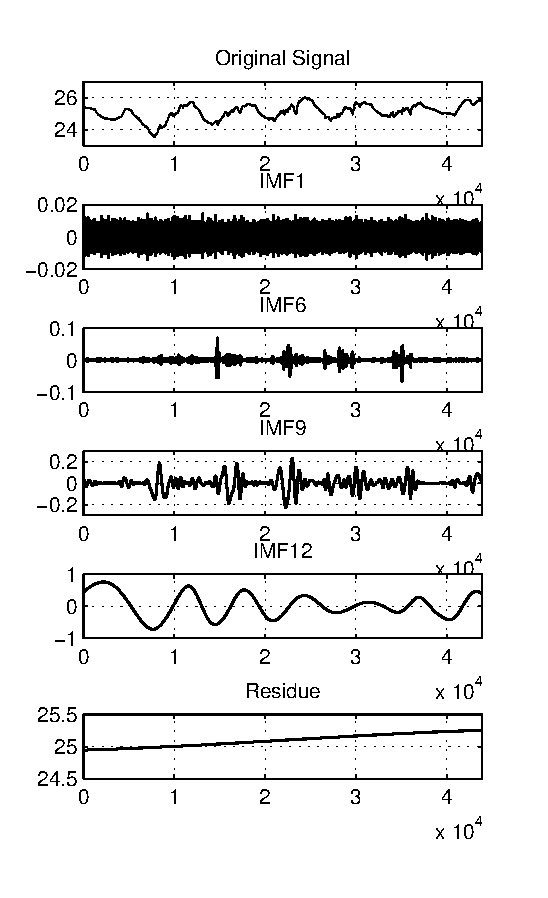
\includegraphics[width=\textwidth]{./fig/emd.eps}
%                 \caption{An example of EMD}
%                 \label{fig:emd}
%   \end{subfigure}
%   \begin{subfigure}{0.32\textwidth}
%                 \centering
%     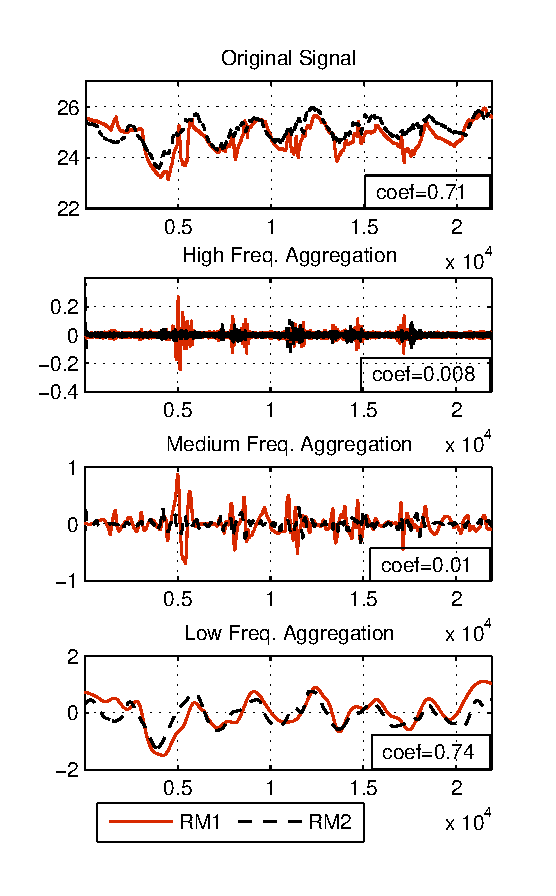
\includegraphics[width=\textwidth]{./fig/imf_aggr1.eps}
%                 \caption{IMFs aggregation}
%                 \label{fig:aggr1}
%   \end{subfigure}
%   \begin{subfigure}{0.32\textwidth}
%                 \centering
%     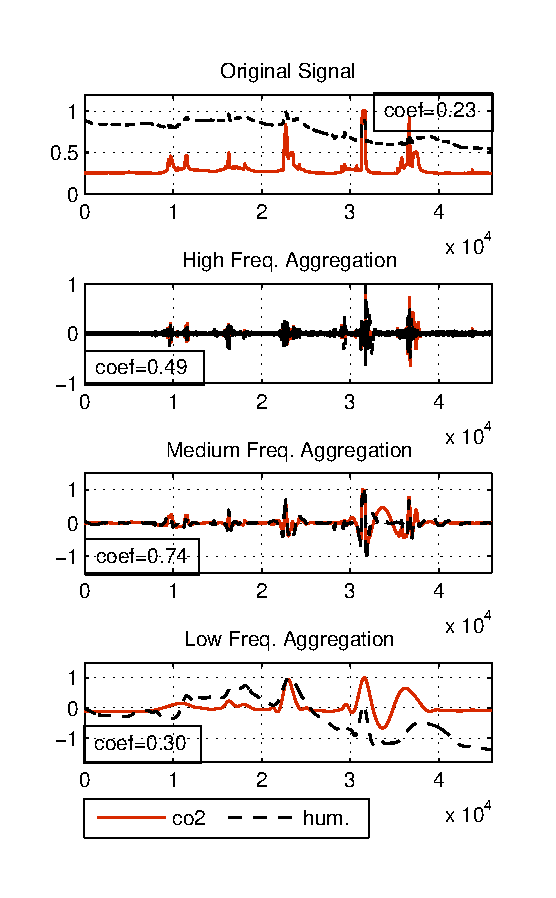
\includegraphics[width=\textwidth]{./fig/imf_aggr2.eps}
%                 \caption{IMFs aggregation}
%                 \label{fig:aggr2}
%   \end{subfigure}
% \caption{(a) EMD decomposes a signal and exposes intrinsic oscillatory components; (b) Aggregation of IMFs within a pre-defined frequency range makes seemingly similar signals from different locations more distinguishable; (c) IMF aggregation makes seemingly distinct signals of different sensors in the same room show high correlation.}
% \end{figure*}

\section{Methodology}
We first describe how we design the feature extraction and explain why the feature set works. Then we discuss the classification technique we adopt as well as detail the training and testing process. In the end, we articulate a solution to identifying potential misclassification for cases where no ground truth labels for sensor types are available.

\subsection{Feature Extraction}
We leverage the information embedded in sensor time series in the time domain. A time domain signal gives the amplitude of a sensor reading and intuitively, different sensor types would in general occupy distinct amplitude bins as demonstrated in Figure~\cite{}. However, sensor readings are subjective to the changes in surroudings therefore sensors of different types can collide in the same amplitude bins. For example, in a rainy season, the humidity in an office can reach the range of 70~80 which is the same as typical temeprature sensor readings. To capture these short term ``events'' as discriminators for Therefore, simply relying on reading amplitude might not be able to effetively differentiate different sensors.

As a summary, the feature extraction procedure goes as follows. First, each single sensor signal is segmented into N non-overlapping X-minute long windows (we will later discuss the choice of window length X). Second, within each time window, we compute the median and variance of the signal, obtaining a vector of medians and a vector of variances. 
\begin{displaymath}
\begin{split}
MED = \{median^{1}, median^{2}, ..., median^{N}\}\\
VAR = \{variance^{1}, variance^{2}, ..., variance^{N}\}
\end{split}
\end{displaymath}
Where N is the number of time windows. The vector $MED$ and $VAR$ reflect short term changes but not all the values are essentially needed for classification. To characterize the two vectors, as a last step, we compute the statistics of each vectors including minimun, maximun, median and variance, resulting in a feature vector of eight elements:
\begin{displaymath}
\begin{split}
F = \{min(MED), max(MED), median(MED), var(MED),\\
 min(VAR), max(VAR), median(VAR), var(VAR)\}
\end{split}
\end{displaymath}
And feature vector $F$ is the input for our classification task.

\subsection{Classification}
After turning all sensor time series into feature vectors, we leverage an ensemble classification technique--random forest--as our classifer to achieve the classification task. Random forest~\cite{RF} works by growing a bunch of classification trees. To classify a new coming object as a feature vector, feed the vector down each of the trees in the forest. Each tree gives a classification, in other words, the tree ``votes" for that class. The forest chooses the class having the most votes over all the trees in the forest. As a quick overview of how each tree is grown in the forest, the process goes as follows:
\begin{enumerate}
\item Sample N instances at random with replacement, from the original data set. These samples will be the training set for growing this particular tree.
\item Specify M feature variables at random out of the total feature vector when growing each node of a tree. And the best split on these M is used to split the node. The value of M is constant during the forest growing.
\item Each tree is grown to the largest extent possible without pruning.
\end{enumerate}
Specifically, we set N the same as the number of instances in the original training set, M the square root of the number of original features and the number of the trees in the forest be 50. Usually these parameters are optimized through cross-validation and we refer interested readers to~\cite{RF} for further deduction and proofs related to random forest.

% \begin{algorithm}[h!]
%  \SetAlgoLined
%  Give signal $X(t)$:\\
%   \While{the \# of maxima in $X(t)$ >3}{
%   (1) identify all the local extrema in $X(t)$\;
%   (2) perform a cubic spline interpolation of maxima to get the upper envelope\;
%   (3) repeat (2) on minima to get the lower envelope\;
%   (4) $h(t) = X(t) - mean((2),(3))$ \;
%   (5) repeat (2)-(4) until $h(t)$ is an IMF\;
%   (6) $X(t) = X(t) - h(t)$, and return the IMF\;
%   }
%  \caption{Empirical Mode Decomposition}
%  \label{alg:emd}
% \end{algorithm}

\subsection{Identifying Misclassification}
It is an easy job to identify misclassification when we have groud truth labels, but in many contexts motivating our solution the ground truth labels are not available, therefore, the identification of potential misclassification would suffer from the absence of ground truth. To identify the potential misclassified instances in our job, we leverage the ensemble of classifiers and make use of a probability-based approach.